% Source: Code/FLIR_Python/architecture_diagrams/system_function_model.tex
\documentclass[border=10pt]{standalone}
\usepackage{tikz}
\usepackage{xcolor}
\usetikzlibrary{shapes.geometric, arrows.meta, positioning, fit, backgrounds, calc}

% USC Color Definitions
\definecolor{uscgarnet}{HTML}{73000a}
\definecolor{uscatlantic}{HTML}{466A9F}
\definecolor{usccongaree}{HTML}{1F414D}
\definecolor{uschorseshoe}{HTML}{65780B}
\definecolor{uscrose}{HTML}{CC2E40}
\definecolor{uscsandstorm}{HTML}{FFF2E3}
\definecolor{uscwarmgrey}{HTML}{676156}

\begin{document}

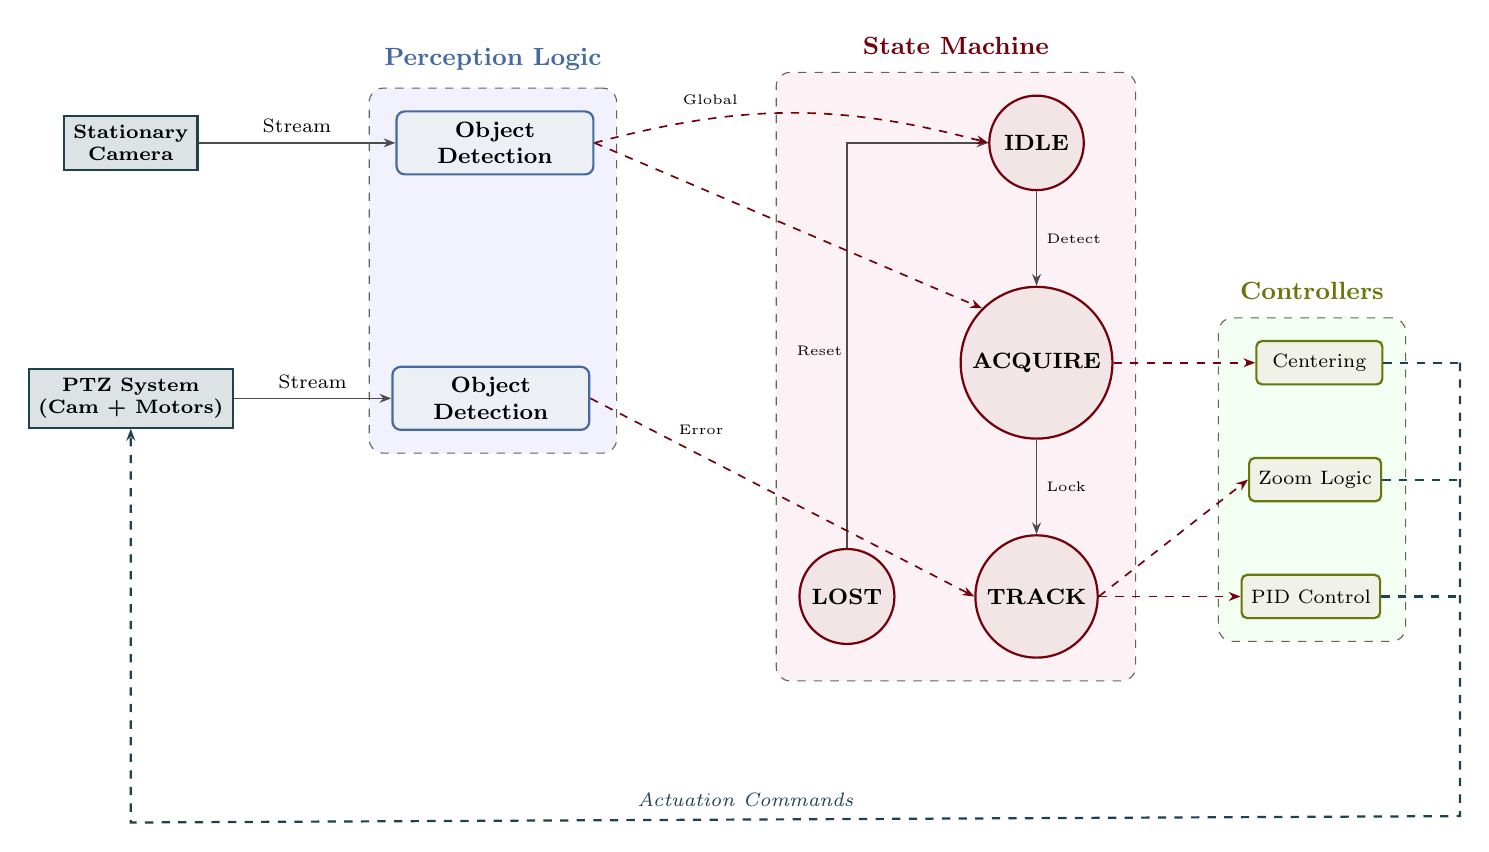
\begin{tikzpicture}[
    % Mimicking styles from system_architecture.tex
    app/.style={rectangle, draw=uscatlantic, fill=uscatlantic!10, thick, minimum width=2.5cm, minimum height=0.8cm, align=center, rounded corners=3pt, font=\footnotesize\bfseries},
    thread/.style={rectangle, draw=uschorseshoe, fill=uschorseshoe!10, thick, minimum width=1.6cm, minimum height=0.55cm, align=center, rounded corners=2pt, font=\scriptsize},
    process/.style={rectangle, draw=uscgarnet, fill=uscgarnet!10, thick, minimum width=1.8cm, minimum height=0.6cm, align=center, rounded corners=3pt, font=\footnotesize\bfseries},
    hardware/.style={rectangle, draw=usccongaree, fill=usccongaree!15, thick, minimum width=1.6cm, minimum height=0.55cm, align=center, font=\scriptsize\bfseries},
    decision/.style={diamond, draw=uscrose, fill=uscrose!10, thick, aspect=2, align=center, font=\scriptsize},
    container/.style={draw=uscwarmgrey, dashed, rounded corners=5pt, inner sep=8pt},
    % Arrow styles
    dataarrow/.style={-{Stealth[length=1.5mm]}, semithick, draw=black!70},
    ipc/.style={-{Stealth[length=1.5mm]}, semithick, draw=uscgarnet, densely dotted},
    hwlink/.style={-{Stealth[length=1.5mm]}, semithick, draw=usccongaree},
    feedback/.style={-{Stealth[length=1.5mm]}, thick, draw=usccongaree, dashed},
]

% ============================================================================
% INPUTS
% ============================================================================
\node[hardware] (statcam) {Stationary\\Camera};
% Combined PTZ Unit (moved slightly lower to make room for feedback)
\node[hardware, below=2.5cm of statcam] (ptzunit) {PTZ System\\(Cam + Motors)};

% ============================================================================
% PERCEPTION FUNCTIONS
% ============================================================================
\node[app, right=2.5cm of statcam] (detstat) {Object\\Detection};
\node[app, right=2cm of ptzunit] (detptz) {Object\\Detection};

% Data flow
\draw[dataarrow] (statcam) -- node[above, font=\scriptsize] {Stream} (detstat);
\draw[dataarrow] (ptzunit) -- node[above, font=\scriptsize] {Stream} (detptz);

% Container
\begin{scope}[on background layer]
    \node[container, fill=blue!5, fit=(detstat)(detptz)] (perceptionbox) {};
\end{scope}
\node[above=0.1cm of perceptionbox, font=\small\bfseries\color{uscatlantic}] {Perception Logic};

% ============================================================================
% TRACKING LOGIC (State Machine)
% ============================================================================
% Using circular nodes for states
\node[process, minimum width=1.2cm, circle, right=5cm of detstat] (idle) {IDLE};
\node[process, minimum width=1.2cm, circle, below=1.2cm of idle] (acquire) {ACQUIRE};
\node[process, minimum width=1.2cm, circle, below=1.2cm of acquire] (track) {TRACK};
\node[process, minimum width=1.2cm, circle, left=1cm of track] (lost) {LOST};

% Container
\begin{scope}[on background layer]
    \node[container, fill=purple!5, fit=(idle)(acquire)(track)(lost)] (logicbox) {};
\end{scope}
\node[above=0.1cm of logicbox, font=\small\bfseries\color{uscgarnet}] {State Machine};

% Transitions
\draw[dataarrow] (idle) -- node[right, font=\tiny] {Detect} (acquire);
\draw[dataarrow] (acquire) -- node[right, font=\tiny] {Lock} (track);
% \draw[dataarrow] (track) -- node[above, font=\tiny] {Timeout} (lost); % Removed based on user request
\draw[dataarrow] (lost) |- (idle);
\node[above left=2.5cm and -0.5cm of lost, font=\tiny] {Reset};


% Inputs to Tracking states
\draw[ipc, dashed, bend left=15] (detstat.east) to (idle.west);
\node[above right=-0.05cm and 1cm of detstat, font=\tiny] {Global};

\draw[ipc, dashed] (detstat.east) to (acquire.north west);

\draw[ipc, dashed] (detptz.east) to (track.west);
\node[above right=-1cm and 1cm of detptz, font=\tiny] {Error};

% ============================================================================
% CONTROL FUNCTIONS
% ============================================================================
\node[thread, right=1.8cm of track] (pid) {PID Control};
\node[thread, right=1.8cm of acquire] (center) {Centering};
\path (pid) -- node[thread] (zoom) {Zoom Logic} (center);

% Container
\begin{scope}[on background layer]
    \node[container, fill=green!5, fit=(pid)(zoom)(center)] (controlbox) {};
\end{scope}
\node[above=0.1cm of controlbox, font=\small\bfseries\color{uschorseshoe}] {Controllers};

% Links to Controllers
\draw[ipc, dashed] (track) -- (pid);
\draw[ipc, dashed] (track.east) -- (zoom.west);
\draw[ipc, dashed] (acquire) -- (center);

% ============================================================================
% FEEDBACK CONTROL LOOPS
% ============================================================================
% Routing control signals BACK to the PTZ unit on the left

% 1. Create a coordinate for the vertical bus to the right of the controllers
\coordinate (bus_x) at ([xshift=1cm]pid.east); 

% 2. Connect individual controllers to the vertical bus (NO ARROWS)
\draw[thick, draw=usccongaree, dashed] (center.east) -- (center.east -| bus_x);
\draw[thick, draw=usccongaree, dashed] (zoom.east) -- (zoom.east -| bus_x);
\draw[thick, draw=usccongaree, dashed] (pid.east) -- (pid.east -| bus_x);

% 3. Draw the main feedback line: Vertical Bus -> Bottom -> Left -> Up (ARROW AT END ONLY)
% Start from the top connection (Center) down to the bottom turn
\draw[feedback] (center.east -| bus_x) -- ([yshift=-2.5cm]pid.south -| bus_x) 
    -- ([yshift=-5cm]ptzunit.south) -- (ptzunit.south);

\node[below right=4.5cm and 5cm of ptzunit, font=\scriptsize\itshape, align=center, color=usccongaree] {Actuation Commands};

\end{tikzpicture}
\end{document}
